% Copyright 2024 Kieran W Harvie. All rights reserved.

\section{Barycentric Coordinates}
Let $P_k$ be the points of an $n$-simplex.
Then for any point $Q$ in the interior there exists a unique set of scalars $\lambda_k$ such that:
\begin{equation*}
\begin{aligned}
	0\leq&\lambda_k\\
	1=&\sum_{k=1}^n\lambda_n\\
	Q=&\sum_{k=1}^nP_n\lambda_n\\
\end{aligned}
\end{equation*}
These scalars are called the barycentric coordinates of the point $Q$.
In this section I will review the $n=2$ case, where the $n$-simplexes are triangles.

\subsection{Etymology}	
This is something that may be obvious to everyone but went over my head for a while.
The `bary' in barycentric isn't from someone named Bary,
but instead comes from the ancient Greek word `barús' meaning heavy,
similar to baryon.

\subsection{Triangles}
Given three 2D points $P_n$ why would we expect the set:
\[\{\lambda_1P_1+\lambda_2P_2+\lambda_3P_3|\lambda_1+\lambda_2+\lambda_3 = 1,\,\lambda_1 \geq 0,\,\lambda_2 \geq 0,\,\lambda_3 \geq 0\}\]
To have anything to do with triangles?
Well consider the function $f:\mathbb{R}^3\rightarrow\mathbb{R}^2$:
\[f(x,y,z) = P_1x+P_2y+P_3z\]
This function is clearly linear:
\begin{equation*}
\begin{aligned}
	&f(ax_0+bx_1,ay_0+by_1,az_0+bz_1)\\
	=&P_1(ax_0+bx_1) + P_2(ay_0+by_1)+P_3(az_0+bz_1)\\
	=&a(P_1x_0+P_2y_0+P_3z_0) + b(P_1x_1+P_2y_1+P_3z_1)\\
	=&af(x_1,y_1,z_1)+bf(x_1,y_1,z_1)\\
\end{aligned}
\end{equation*}
Meaning it sends line segments to lines segments:
\[f(At+B(1-t)) = f(A)t+f(B)(1-t)\] 
(Or to a single point point if $f(A)=f(B)$.)
\\

Now,
consider the subset of $\mathbb{R}^3$ such that $x,y,z\geq0$ and $x+y+z=1$.
This is set is an equilateral triangle spanning the points $(1,0,0),\,(0,1,0)$ and $(0,0,1)$,
with the image of these points being the points $P_n$.
This subset is by definition the span of the barycentric coordinates.
\\

These result combined show that function maps the boundary of the equilateral triangle to $P_1P_2P_3$.
\\

But what about the interior?
Is it mapped to the interior or exterior of $P_1P_2P_3$?
To see why it's the interior consider the following result:

\subsection{Area coordinates}
\begin{center}
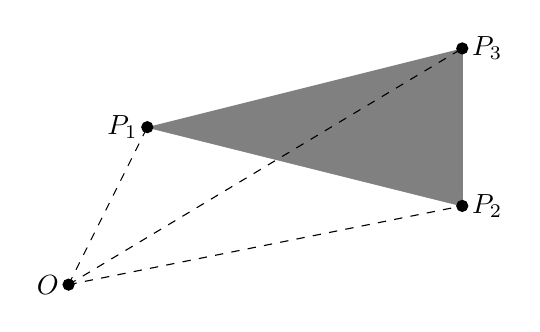
\begin{tikzpicture}[every node/.style={black}]
	\coordinate (O) at (0,0);
	\coordinate (P1) at (1,2);
	\coordinate (P2) at (5,1);
	\coordinate (P3) at (5,3);


	\filldraw[gray] (P1) -- (P2) -- (P3);

	\draw[dashed] (O) -- (P1);
	\draw[dashed] (O) -- (P2);
	\draw[dashed] (O) -- (P3);

	\filldraw (O) node[left] {$O$} circle (2pt);
	\filldraw (P1) node[left] {$P_1$} circle (2pt);
	\filldraw (P2) node[right] {$P_2$} circle (2pt);
	\filldraw (P3) node[right] {$P_3$} circle (2pt);
\end{tikzpicture}
\end{center}
The (unsigned) area of a triangle with points $P_1P_2P_3$ is given by:
\begin{equation*}
\begin{aligned}
	&\frac{1}{2}\left|\begin{vmatrix} x_1&x_2\\y_1&y_2\end{vmatrix} + \begin{vmatrix} x_2&x_3\\y_2&y_3 \end{vmatrix} + \begin{vmatrix} x_3&x_1\\y_3&y_1\end{vmatrix}\right|\\
	=&\frac{1}{2}(x_1(y_3-y_2)+x_2(y_1-y_3)+x_3(y_2-y_1))\\
\end{aligned}
\end{equation*}
This follows directly from the determinant being the signed area of the parallelogram spanned by its column vectors and can be rewritten, to isolate $P_1$, as:
\[\frac{1}{2}\big|x_1(y_3-y_2)-y_1(x_3-x_2)+x_3y_2-x_2y_3\big|\]
Let $Q$ have barycentric coordinates $(\lambda_1,\lambda_2,\lambda_3)$ and consider the area of the triangle $P_2P_3Q$:
\[\frac{1}{2}(\big|\lambda_1x_1+ \lambda_2x_2 + \lambda_3x_3)(y_3-y_2)-(\lambda_1y_1+ \lambda_2y_2 + \lambda_3y_3)(x_3-x_2)+x_3y_2-x_2y_3\big|\]
Considering just the first part shows that the like term, $x_ny_m$ where $n=m$, cancel to give:
\begin{equation*}
\begin{aligned}
	&(\lambda_1x_1+ \lambda_2x_2 + \lambda_3x_3)(y_3-y_2)-(\lambda_1y_1+ \lambda_2y_2 + \lambda_3y_3)(x_3-x_2)\\
	=&\lambda_1(x_1(y_3-y_2)-y_1(x_3-x_2))+ (\lambda_2x_2 + \lambda_3x_3)(y_3-y_2)-(\lambda_2y_2 + \lambda_3y_3)(x_3-x_2)\\
	=&\lambda_1(x_1(y_3-y_2)-y_1(x_3-x_2))+ \lambda_2(x_2y_3-x_3y_2) +\lambda_3(x_2y_3-x_3y_2)\\
	=&\lambda_1(x_1(y_3-y_2)-y_1(x_3-x_2))+ (1-\lambda_1)(x_2y_3-x_3y_2)\\
\end{aligned}
\end{equation*}
And hence and area of the triangle as:
\[\frac{\lambda_1}{2}\big|x_1(y_3-y_2)-y_1(x_3-x_2)+x_3y_2-x_2y_3\big|\]
This is why barycentric coordinates for triangles are also called area coordinates.
Because the first coordinate is the ratio of the area of the total triangle to $P_2P_3Q$,
and likewise for the other coordinates.
\\

It also flows that for this to be valid for all $\lambda_n$ that $Q$ is internal and unique.

% Trilinear conversion?

%The altitude of $P_1$ is perpendicular to $\overline{P_2P_3}$ giving it a gradient of:
%\[-\left(\frac{y_3-y_2}{x_3-x_2}\right)^{-1}= \frac{x_2-x_3}{y_3-y_2}\]
%Hence the foot lies at the intersection of:
%\begin{equation*}
%\begin{aligned}
%	0=&(y_3-y_2)(x-x_2)-(x_3-x_2)(y-y_2)\\
%	0=&(x_3-x_2)(x-x_1)+(y_3-y_2)(y-y_1)\\
%\end{aligned}
%\end{equation*}
%Giving the cool relations:
%\begin{equation*}
%\begin{aligned}
%	0=&(y_3-y_2)^2(x-x_2)+(x_3-x_2)^2(x-x_1)+(x_3-x_2)(y_3-y_2)(y_2-y_1)\\
%	0=&(x_3-x_2)^2(y-y_2)-(y_3-y_2)^2(y-y_1)+(x_3-x_2)(y_3-y_2)(x_2-x_1)\\
%\end{aligned}
%\end{equation*}
%
